A lo largo de todo el capítulo supondremos que los grafos en cuestión son localmente finitos y sin vértices aislados.
\begin{Prop}
   Sea $G=(V,E)$ un grafo. El conjunto $\mathcal{S}_{\mathcal{A},G}:=\left\lbrace A_x\mid x\in V\right\rbrace$ es subbase para una topología sobre $V$.
\end{Prop}
\begin{proof}
   Tenemos que $\mathcal{S}_{\mathcal{A},G}$ es una colección de subconjuntos de $V$. Para cualquier $v\in V$, como $G$ no tiene vértices aislados, existe $u\in V$ tal que $v\in A_u$, de modo que $v\in\bigcup_{x\in V}A_x$. Por tanto $\bigcup_{x\in V}A_x=V$ y $\mathcal{S}_{\mathcal{A},G}$ es subbase para una topología sobre $V$.
\end{proof}
Como pudimos ver, la condición de no tener vértices aislados es clave para que $\mathcal{S}_{\mathcal{A},G}$ sea subbase para una topología sobre $V$, pues si $G$ tuviera algún vértice aislado $v$, se tendría $v\in V$ pero $v\notin\bigcup_{x\in V}A_x$, dado que $v\notin A_x$ para todo $x\in V$.
\begin{Def}
   Sea $G=(V,E)$ un grafo. La topología generada por la subbase $\mathcal{S}_{\mathcal{A},G}$, denotada por $\tau_{\mathcal{A},G}:=\tau_{\mathcal{S}_{\mathcal{S},G}}$, es llamada la \textbf{topología de adyacencia de $G$}.  
\end{Def}
\begin{Prop}
   \phantom{o}
   \begin{itemize}
      \item[1.] Para todo $n\ge 2$, la topología de adyacencia de $K^n$ es discreta.
      \item[2.] Para todo $n\ge 5$, la topología de adyacencia de $C^n$ es discreta.
      \item[3.] Para todo $n\ge 3$, la topología de adyacencia de $P^n$ es no discreta.
      \item[4.] Para cualesquiera $n,m\ge 1$, la topología de adyacencia del grafo bipartito completo $K_{n,m}$ es $\{\emptyset, V, A, B\}$, donde $V=V\left( K_{n,m}\right)$ y $A$ y $B$ son las particiones de $V$.
   \end{itemize}
\end{Prop}
\begin{proof}
   \phantom{o}
   \begin{itemize}
      \item[1.] Sea $n\ge 2$ cualquiera. Denotemos $V\left( K^n\right)=\{v_1,\dots, v_n\}$. Sea $i\in\{1,\dots, n\}$ cualquiera. Basta ver que $\left\lbrace v_i\right\rbrace\in \tau_{\mathcal{A},K^n}$ Veamos que $\left\lbrace v_i\right\rbrace=\bigcap_{1\le j\le n, j\ne i}A_{v_j}$. Por la definición de $K^n$ se tiene $v_i\in A_{v_j}$ para todo $j$ tal que $1\le j\le n$ y $j\ne i$. Por tanto $v_i\in\bigcap_{1\le j\le n, j\ne i} A_{v_j}$ y $\left\lbrace v_i\right\rbrace\subseteq \bigcap_{1\le j\le n, j\ne i} A_{v_j}$. Ahora, dado cualquier $k$ con $1\le k\le n$ y $k\ne i$ se tiene $v_k\notin A_{v_k}$, luego $v_k\notin \bigcap_{1\le j\le n, j\ne i} A_{v_j}$. Con esto, $V\setminus \left\lbrace v_i\right\rbrace\subseteq V\setminus \bigcap_{1\le j\le n, j\ne i} A_{v_j}$, es decir $\bigcap_{1\le j\le n, j\ne i} A_{v_j} \subseteq \left\lbrace v_i\right\rbrace$. Obtenemos así $\left\lbrace v_i\right\rbrace=\bigcap_{1\le j\le n, j\ne i} A_{v_j}$. Como $\left\lbrace v_i\right\rbrace$ es una intersección finita de elementos de $\mathcal{S}_{\mathcal{A},K^n}$, se tiene $\left\lbrace v_i\right\rbrace\in \tau_{\mathcal{A},K^n}$.
      \item[2.] Sea $n\ge 5$ cualquiera. Denotemos $V\left( C^n\right)=\left\lbrace v_0,\dots,v_{n-1}\right\rbrace$. Basta ver que $\left\lbrace v_i\right\rbrace\in\tau_{\mathcal{A},C^n}$ para cualquier $i\in\{0,\dots,n-1\}$.
         \begin{figure}[H]
\centering
\resizebox{0.25\textwidth}{!}{
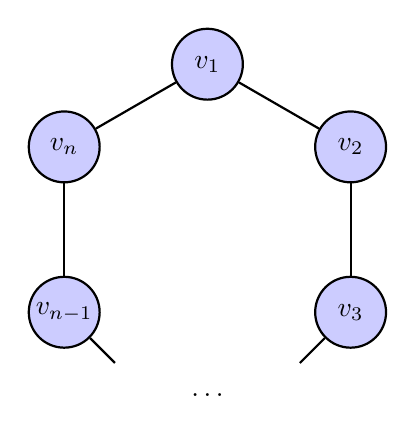
\begin{tikzpicture}[
  scale=0.7,
  vnode/.style={circle, fill=blue!20, draw=black, thick, inner sep=0pt, minimum size=0.9cm}
]

  % Vértices iniciales (lado derecho)
  \node[vnode] (v1) at (90:3) {$v_1$};
  \node[vnode] (v2) at (30:3) {$v_2$};
  \node[vnode] (v3) at (-30:3) {$v_3$};

  % Vértices finales (lado izquierdo)
  \node[vnode] (vn1) at (210:3) {$v_{n-1}$};
  \node[vnode] (vn) at (150:3) {$v_n$};

  % Puntos suspensivos y nodos auxiliares para continuar las aristas en la parte inferior
  \node[draw=none, fill=none] (dots) at (-90:3) {$\dots$};
  \node[draw=none, fill=none, minimum size=0pt] (v3_inv) at (-60:3) {};
  \node[draw=none, fill=none, minimum size=0pt] (vn1_inv) at (-120:3) {};

  % Aristas continuas visibles
  \draw[thick] (v1) -- (v2);
  \draw[thick] (v2) -- (v3);
  \draw[thick] (vn1) -- (vn);
  \draw[thick] (vn) -- (v1); % Arista que cierra el ciclo entre v_n y v_1

  % Aristas que se dirigen hacia la elipsis inferior
  \draw[thick] (v3) -- (v3_inv);
  \draw[thick] (vn1_inv) -- (vn1);

\end{tikzpicture}}
\caption{El grafo $C^n$}
\label{fig:ciclo_n}
\end{figure}

         Para todo $i\in\{0,\dots,n-1\}$ se tiene $A_{v_i}=\left\lbrace v_{(i-1)\bmod n},v_{(i+1)\bmod n}\right\rbrace$ y por tanto $A_{v_{(i-1)\bmod n}}=\left\lbrace v_{(i-2)\bmod n},v_i\right\rbrace$ y $A_{v_{(i+1)\bmod n}}=\left\lbrace v_i,v_{(i+2)\bmod n}\right\rbrace$. Como $n\ge 5$ se tiene $(i-2)\bmod n\ne (i+2)\bmod n$, de modo que $v_{(i-2)\bmod n}\ne v_{(i+2)\bmod n}$ y por tanto $\left\lbrace v_i\right\rbrace=A_{v_{(i-1)\bmod n}}\cap A_{v_{(i+1)\bmod n}}$. Como $\left\lbrace v_i\right\rbrace$ es una intersección finita de elementos de $\mathcal{S}_{\mathcal{A},C^n}$ entonces $\left\lbrace v_i\right\rbrace\in\tau_{\mathcal{A},C^n}$.
      \item[3.] Sea $n\ge 3$ cualquiera.
         \begin{figure}[H]
\centering
\resizebox{0.45\textwidth}{!}{
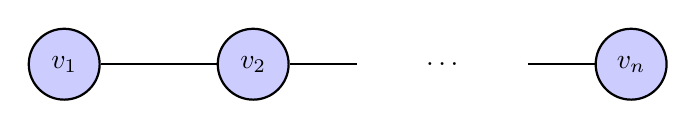
\begin{tikzpicture}[
  scale=1.2,
  vnode/.style={circle, fill=blue!20, draw=black, thick, inner sep=0pt, minimum size=0.9cm}
]

  % Posicionamiento de vértices horizontales
  \node[vnode] (v1) at (0, 0) {$v_1$};
  \node[vnode] (v2) at (2, 0) {$v_2$};
  
  % Puntos suspensivos y nodos auxiliares para conectar las aristas
  \node[draw=none, fill=none] (dots) at (4, 0) {$\dots$};
  \node[draw=none, fill=none, inner sep=0pt, minimum size=0pt] (v2_out) at (3.1, 0) {};
  \node[draw=none, fill=none, inner sep=0pt, minimum size=0pt] (vn_in) at (4.9, 0) {};

  % Vértice final
  \node[vnode] (vn) at (6, 0) {$v_n$};

  % Arista continua entre v1 y v2
  \draw[thick] (v1) -- (v2);

  % Aristas de entrada/salida hacia la elipsis
  \draw[thick] (v2) -- (v2_out);
  \draw[thick] (vn_in) -- (vn);

\end{tikzpicture}}
\caption{El grafo $P^n$}
\label{fig:camino_n}
\end{figure}

         Veamos que $\left\lbrace v_1\right\rbrace\notin\tau_{\mathcal{A},P^n}$. Sea $U\in\tau_{\mathcal{A},P^n}$ cualquiera con $v_1\in U$. Basta probar que $v_3\in U$. Tenemos $A_{v_1}=\left\lbrace v_2\right\rbrace$, $A_{v_i}=\left\lbrace v_{i-1},v_{i+1}\right\rbrace$ para cualquier $i$ con $2\le i\le n-1$ y $A_{v_n}=\left\lbrace v_{n-1}\right\rbrace$. Existe $B\subseteq\mathcal{B}_{\mathcal{S}_{\mathcal{A},P^n}}$ tal que $U=\bigcup B$. Entonces $v_1\in S$ para algún $S\in B$. Como en particular $S\in \mathcal{B}_{\mathcal{S}_{\mathcal{A},P^n}}$, luego $S=\bigcap_{j=1}^{m}A_{v_{i_j}}$ para algún $m\in \mathbb{Z}^+$ y con $i_j\in\{1,\dots,n\}$ para todo $j\in\{1,\dots,m\}$. Tenemos que $v_1\in A_{v_{i_j}}$ para todo $j\in\{1,\dots,m\}$. Como $v_1\in A_{v_2}$ y $v_1\notin A_{v_k}$ para todo $k\in\{3,\dots,n\}$ entonces $A_{v_{i_j}}=A_{v_2}$ para todo $j\in\{1,\dots,m\}$, de modo que $A_{v_2}=S\subseteq U$ y por tanto $v_3\in U$.
      \item[4.] Sean $n,m\ge 1$ cualesquiera. Dado $a\in A$ se tiene $A_a=B$, y dado $b\in B$ se tiene $A_b=A$. Por tanto $\mathcal{S}_{\mathcal{A},K_{n,m}}=\left\lbrace A,B\right\rbrace$. Como $A\cap B=\emptyset$, tenemos $\mathcal{B}_{\mathcal{S}_{\mathcal{A},K_{n,m}}}=\left\lbrace A,B\right\rbrace$, y como $A\cup B=V$ entonces $\tau_{\mathcal{A},k_{n,m}}=\left\lbrace \emptyset,V,A,B\right\rbrace$. 
   \end{itemize}
\end{proof}
\begin{Obs}
   Se tiene que $K^1=P^1$ está formado por un solo vértice (que por tanto es aislado), de modo que no tiene definida topología de adyacencia. Además $C^3=K^3$, y por tanto $C^3$ tiene topología de adyacencia discreta. En la \Cref{sec:computacional_adyacencia} calcularemos la topología de adyacencia de $C^4$ y veremos que no es discreta. 
\end{Obs}
